\documentclass[11pt,a4paper]{article}

% ===== Paquetes requeridos por la guía GA-SUM-03 =====
\usepackage[utf8]{inputenc}
\usepackage[T1]{fontenc}
\usepackage[spanish]{babel}
\usepackage{booktabs}      % tablas
\usepackage{array}         % columnas p{} con alineación personalizada
\usepackage{ragged2e}      % \RaggedRight para columnas p{} sin huecos (evita underfull hbox)
\usepackage{csquotes}      % recomendado por babel/polyglossia junto con biblatex
\usepackage{listings}      % código
\usepackage{xcolor}        % colores (código, diagramas)
\usepackage{graphicx}      % figuras
\usepackage{tikz}          % diagrama de secuencia Raft (elaboración propia)
\usetikzlibrary{positioning, arrows.meta, calc}
\usepackage{float}         % posición [H] para figuras y tablas
\usepackage[style=ieee,backend=biber]{biblatex} % referencias IEEE
\usepackage{amsmath}       % ecuaciones
\usepackage{amssymb}       % símbolos matemáticos adicionales (\ltimes, \rtimes)
\usepackage{hyperref}      % hipervínculos
\usepackage{geometry}
\geometry{margin=2.5cm}

\addbibresource{referencias.bib}

% Columna tipo p{} con alineación RaggedRight: evita los huecos excesivos
% (underfull hbox) que deja la justificación completa en columnas angostas,
% y permite el salto de línea que las columnas l/c/r no ofrecen (evita overfull hbox).
\newcolumntype{P}[1]{>{\RaggedRight\arraybackslash}p{#1}}

\definecolor{codebg}{RGB}{245,245,245}
\lstdefinelanguage{yaml}{
  keywords={image, container_name, hostname, command, ports, volumes, networks,
            environment, driver, name, services, version, healthcheck, test,
            interval, timeout, retries, start_period, mem_limit},
  sensitive=true,
  comment=[l]{\#},
  morestring=[b]",
  morestring=[b]',
}
\lstset{
  backgroundcolor=\color{codebg},
  basicstyle=\ttfamily\footnotesize,
  breaklines=true,
  breakatwhitespace=false,
  frame=single,
  numbers=left,
  numberstyle=\tiny,
  showstringspaces=false,
  tabsize=2,
  literate=
    {á}{{\'a}}1 {é}{{\'e}}1 {í}{{\'i}}1 {ó}{{\'o}}1 {ú}{{\'u}}1
    {Á}{{\'A}}1 {É}{{\'E}}1 {Í}{{\'I}}1 {Ó}{{\'O}}1 {Ú}{{\'U}}1
    {ñ}{{\~n}}1 {Ñ}{{\~N}}1
}

\title{Implementaci\'on y Verificaci\'on de un Cl\'uster de Base de Datos Distribuida con CockroachDB aplicado al PFC\\
\large GA-SUM-03 / PE-U3 -- Cl\'uster BDD aplicado al PFC ACC -- Soporte T\'ecnico ISP}
\author{}
\date{}

\begin{document}

\maketitle

\begin{center}
\begin{tabular}{ll}
\toprule
\textbf{C\'odigo de equipo} & D \\
\textbf{PFC de referencia} & ACC --- Soporte T\'ecnico ISP \\
\textbf{T\'itulo del sistema} & Sistema de Gesti\'on de Solicitudes para Soporte T\'ecnico de Internet \\
\bottomrule
\end{tabular}
\end{center}

\begin{center}
\begin{tabular}{P{5.2cm}P{4.3cm}P{4.3cm}}
\toprule
\textbf{Integrante} & \textbf{Rol} & \textbf{PFC de origen} \\
\midrule
Aucatoma Celorio, Jhinson Stalyn & Responsable de documentaci\'on & AGLS -- TiendaTech \\
Alvarez Parraga, Jeremy Alexis & Responsable de calidad & ACC -- Soporte T\'ecnico ISP \\
Carpio Mendoza, Carlos Jos\'e & L\'ider de desarrollo & ACC -- Soporte T\'ecnico ISP \\
\bottomrule
\end{tabular}
\end{center}

\paragraph{Justificaci\'on de la elecci\'on del PFC (m\'aximo 100 palabras).}
Se eligi\'o el dominio ACC porque el ticket de soporte tiene un dato muy
natural para dividir la informaci\'on: la zona geogr\'afica del cliente
(centro, norte o sur de Quevedo). En la vida real, un t\'ecnico casi siempre
revisa solo los tickets de su propia zona, as\'i que dividir la tabla por esa
columna no es un ejercicio forzado, sino algo que tendr\'ia sentido usar en
producci\'on. Adem\'as, la cantidad de tickets que se registran y actualizan
constantemente permite poner a prueba de forma clara tanto la tolerancia a
fallos como el rendimiento del cl\'uster distribuido.

\begin{abstract}
Este informe documenta la implementaci\'on, verificaci\'on y evaluaci\'on de un
cl\'uster de base de datos distribuida de tres nodos con CockroachDB, aplicado
al esquema de datos del sistema de gesti\'on de solicitudes de soporte t\'ecnico
de Internet (PFC ACC). Se desarrolla el fundamento te\'orico de bases de datos
distribuidas exigido por la gu\'ia (arquitecturas, fragmentaci\'on y
replicaci\'on, control de concurrencia y consenso, y el espectro de
consistencia, disponibilidad y PACELC), se describe la configuraci\'on del
cl\'uster en contenedores Docker y la estrategia de fragmentaci\'on horizontal
de la tabla \texttt{tickets} por zona geogr\'afica de atenci\'on
(centro, norte y sur de Quevedo), se verifica experimentalmente la
tolerancia a fallos mediante el algoritmo de consenso Raft, y se presenta un
an\'alisis comparativo cuantitativo de rendimiento entre el cl\'uster
distribuido y una instancia de nodo \'unico sobre cinco consultas
representativas del dominio. Los resultados muestran que la ventaja del
cl\'uster distribuido no es uniforme: resulta favorable en consultas con
carga de c\'omputo significativa (agregaciones, \emph{joins}), mientras que
el nodo \'unico es m\'as r\'apido en lecturas puntuales por clave primaria,
donde el costo fijo de coordinaci\'on distribuida no tiene contrapartida en
paralelismo real.
\end{abstract}

\begin{center}
\textbf{Abstract}
\end{center}

\noindent This report documents the implementation, verification, and
evaluation of a three-node distributed database cluster built with
CockroachDB, applied to the data schema of a ticket management system for
Internet technical support (PFC ACC). The theoretical foundation of
distributed databases required by the practice guide is developed,
covering distributed architectures, fragmentation and replication,
distributed concurrency control and consensus, and the
consistency--availability--PACELC spectrum. The cluster configuration in
Docker containers and the horizontal fragmentation strategy applied to the
\texttt{tickets} table by geographic service zone (Quevedo's centro, norte,
and sur) are described, fault tolerance is verified experimentally through
the Raft consensus algorithm, and a quantitative comparative performance
analysis is presented between the distributed cluster and a single-node
instance across five representative queries of the domain. The results
show that the advantage of the distributed cluster is not uniform: it is
favorable for queries with significant computational load (aggregations,
joins), whereas the single node is faster for point reads by primary key,
where the fixed cost of distributed coordination has no counterpart in
real parallelism.

\section{Introducci\'on}
\label{sec:introduccion}

Las bases de datos distribuidas (BDD) han pasado de ser una alternativa de
nicho a convertirse en el est\'andar de facto para sistemas que exigen alta
disponibilidad, escalabilidad horizontal y tolerancia a fallos
geogr\'aficos~\cite{kleppmann2017,ozsu2020}. CockroachDB es un representante
moderno de la familia \emph{NewSQL}: combina la interfaz y las garant\'ias
transaccionales de una base de datos relacional tradicional con la
arquitectura de fragmentaci\'on y replicaci\'on autom\'atica propia de los
sistemas NoSQL de gran escala, apoy\'andose en el algoritmo de consenso
Raft~\cite{ongaro2014} para coordinar las r\'eplicas de cada fragmento de
datos~\cite{taft2020}.

Este trabajo aplica estos conceptos al Proyecto Fin de Curso (PFC) del equipo
ACC (Soporte T\'ecnico ISP), cuyo n\'ucleo funcional --materializado en el
bounded context de Gesti\'on de Tickets y su microservicio
\texttt{ticket-service}-- es la gesti\'on del ciclo de vida de solicitudes de
soporte t\'ecnico de Internet, distribuidas en tres zonas operativas de la
ciudad de Quevedo. El objetivo de esta pr\'actica es doble: (a) demostrar
experimentalmente que la fragmentaci\'on horizontal y la replicaci\'on
configuradas se comportan seg\'un la teor\'ia --en particular, que el sistema
sobrevive a la ca\'ida de un nodo sin p\'erdida de disponibilidad ni de
datos-- y (b) cuantificar el costo/beneficio real de la distribuci\'on frente
a una instancia de nodo \'unico, en vez de asumirlo por argumento de
autoridad.

A diferencia del resto de la arquitectura de microservicios del PFC ACC
--donde cada bounded context (Autenticaci\'on, Tickets, Notificaciones,
Inteligencia Artificial, Reportes) posee su propia base de datos siguiendo el
patr\'on \emph{database-per-service}-- esta pr\'actica no introduce un sexto
motor de base de datos independiente, sino que verifica c\'omo se comportar\'ia
el esquema del microservicio \texttt{ticket-service} si, en lugar de una
\'unica instancia PostgreSQL, se desplegara sobre un cl\'uster distribuido de
tres nodos. Esto permite ejercitar sobre datos y consultas reales del dominio
los conceptos de fragmentaci\'on, replicaci\'on y consenso que la sola
arquitectura de microservicios --con bases de datos independientes pero cada
una internamente centralizada-- no pone a prueba por s\'i sola.

El resto del documento se organiza as\'i: la Secci\'on~\ref{sec:teoria}
desarrolla el fundamento te\'orico exigido por la gu\'ia; la
Secci\'on~\ref{sec:procedimiento} documenta el procedimiento aplicado con
evidencia reproducible; la Secci\'on~\ref{sec:resultados} presenta los
resultados experimentales y el an\'alisis comparativo de rendimiento; la
Secci\'on~\ref{sec:analisis-critico} discute cr\'iticamente los hallazgos y
sus limitaciones metodol\'ogicas; y la Secci\'on~\ref{sec:conclusiones} cierra
con las conclusiones.

\section{Fundamento te\'orico}
\label{sec:teoria}

\subsection{Fundamentos y arquitecturas de bases de datos distribuidas}

Una base de datos distribuida (BDD) es una colecci\'on de datos l\'ogicamente
interrelacionados que se encuentran f\'isicamente dispersos en distintos sitios
de una red de computadoras, de modo que cada sitio cuenta con un grado de
autonom\'ia de procesamiento y, sin embargo, coopera con los dem\'as para dar al
usuario la impresi\'on de estar interactuando con un \'unico sistema
centralizado~\cite{ozsu2020,date2000}. El sistema de gesti\'on de bases de datos
distribuidas (SGBDD) es el software que administra esa colecci\'on de datos y
provee las facilidades de acceso necesarias para que dicha distribuci\'on sea,
en la mayor medida posible, transparente al usuario~\cite{ozsu2020,date2000}. Esta
definici\'on es relevante para el PFC ACC -- Soporte T\'ecnico ISP, dado que la
pr\'actica exige llevar el esquema de datos del microservicio
\texttt{ticket-service} (tablas como \texttt{tickets} y
\texttt{technicians}) a un cl\'uster de tres nodos, es decir,
transformar una base de datos originalmente centralizada en una BDD en el
sentido estricto del t\'ermino.

Date propuso, a partir del principio fundamental de que ``un sistema distribuido
deber\'ia comportarse, desde la perspectiva del usuario, exactamente igual que un
sistema no distribuido'', un conjunto de doce objetivos que sirven como marco de
referencia para caracterizar cualquier SGBDD~\cite{date2000}. Estos objetivos son:
(1) autonom\'ia local, (2) no dependencia de un sitio central, (3) operaci\'on
continua, (4) independencia de ubicaci\'on, (5) independencia de fragmentaci\'on,
(6) independencia de replicaci\'on, (7) procesamiento de consultas distribuidas,
(8) administraci\'on de transacciones distribuidas, (9) independencia de
hardware, (10) independencia de sistema operativo, (11) independencia de red y
(12) independencia de SGBD~\cite{date2000,ozsu2020}. Özsu y Valduriez retoman este mismo
marco al describir la transparencia de distribuci\'on como el objetivo central
de todo SGBDD, y precisan que ninguno de estos doce objetivos se alcanza jam\'as
de forma absoluta en un sistema real, sino que cada implementaci\'on los satisface
en distinto grado~\cite{ozsu2020}. Para el cl\'uster de CockroachDB de la
pr\'actica, los objetivos m\'as exigidos son la independencia de fragmentaci\'on
(objetivo 5) y la administraci\'on de transacciones distribuidas (objetivo 8),
ya que ambos se verifican expl\'icitamente al ejecutar \texttt{SHOW RANGES}
sobre la tabla \texttt{tickets} y al
comprobar la continuidad del servicio ante la ca\'ida de un nodo.

En cuanto a las arquitecturas de referencia, la literatura distingue al menos
tres modelos. La arquitectura \emph{cliente-servidor} separa con claridad las
responsabilidades: los servidores administran los datos y procesan las
consultas, mientras que los clientes proveen la interfaz y la l\'ogica de
aplicaci\'on, de forma similar a como un sistema centralizado at\'endido por
m\'ultiples clientes remotos~\cite{ozsu2020,coulouris2012}. La arquitectura
\emph{colaborativa} (tambi\'en llamada de igual a igual o \emph{peer-to-peer})
elimina esa distinci\'on funcional: cada sitio ejecuta una instancia completa
del SGBDD y coopera con los dem\'as en pie de igualdad para resolver una
consulta global, que es exactamente el modelo que sigue un cl\'uster de
CockroachDB, en el que cualquier nodo puede recibir una petici\'on y coordinar
su ejecuci\'on~\cite{ozsu2020,coulouris2012}. Finalmente, la arquitectura de \emph{middleware}
aparece cuando los sitios integrantes ejecutan SGBD distintos y aut\'onomos
(un sistema multibase de datos o federado); en este caso se introduce una capa
de mediadores y envoltorios (\emph{mediator/wrapper}) que traduce un esquema
conceptual global a los esquemas locales heterog\'eneos de cada
fuente~\cite{ozsu2020,valduriez2011}.

Un SGBDD debe adem\'as ofrecer distintas formas de transparencia, entendidas
como la capacidad del sistema de ocultar al usuario los detalles de
implementaci\'on de la distribuci\'on. La \emph{transparencia de
fragmentaci\'on} permite formular consultas sobre las relaciones completas sin
conocer c\'omo est\'an particionadas f\'isicamente~\cite{ozsu2020,kleppmann2017}. La
\emph{transparencia de replicaci\'on} permite operar como si existiera una
\'unica copia de cada dato, aun cuando existan varias r\'eplicas~\cite{ozsu2020,kleppmann2017}.
La \emph{transparencia de ubicaci\'on} evita que el usuario deba conocer el
sitio f\'isico donde reside cada fragmento o r\'eplica~\cite{ozsu2020,coulouris2012}. La
\emph{transparencia de acceso} permite invocar operaciones locales y remotas
con la misma interfaz~\cite{coulouris2012,vansteen2017}. La \emph{transparencia de
concurrencia} garantiza que la ejecuci\'on simult\'anea de varias
transacciones no altere el resultado que cada una percibe, como si se
ejecutara en solitario~\cite{coulouris2012,ozsu2020}. La \emph{transparencia
de fallos} oculta, en la medida de lo posible, la ca\'ida de un nodo o de un
enlace de comunicaci\'on~\cite{coulouris2012,vansteen2017}. La \emph{transparencia
de escalabilidad} permite incorporar nuevos nodos sin que ello obligue a
rediseñar las aplicaciones existentes~\cite{coulouris2012,vansteen2017}. Por \'ultimo, la
\emph{transparencia de evoluci\'on} (una extensi\'on distribuida de la
independencia l\'ogica de datos) permite modificar el esquema global o la
codificaci\'on de los registros a lo largo del tiempo sin romper la
compatibilidad con las aplicaciones cliente ya desplegadas~\cite{kleppmann2017,ozsu2020}.
Estas ocho transparencias se verificar\'an de forma pr\'actica en la
Secci\'on~\ref{sec:procedimiento} al comprobar que las consultas SQL sobre la
tabla principal del PFC no requieren modificaci\'on alguna tras aplicar la
fragmentaci\'on ni durante la ca\'ida de un nodo del cl\'uster.

Finalmente, es necesario distinguir entre BDD homog\'eneas y heterog\'eneas.
Un sistema homog\'eneo utiliza el mismo motor de SGBD, el mismo modelo de
datos y, en general, el mismo lenguaje de consulta en todos sus sitios, lo
que simplifica de forma considerable el procesamiento de consultas
distribuidas y la administraci\'on de transacciones~\cite{ozsu2020,date2000}. Un
sistema heterog\'eneo, en cambio, integra motores distintos y aut\'onomos
(por ejemplo, un sistema relacional junto con un almac\'en documental), lo
que exige mecanismos adicionales de traducci\'on de esquemas y de
resoluci\'on de conflictos sem\'anticos entre fuentes~\cite{ozsu2020,valduriez2011}.
El cl\'uster de tres nodos CockroachDB que se implementa en esta pr\'actica
corresponde a una BDD homog\'enea, ya que los tres nodos ejecutan el mismo
motor y comparten un \'unico esquema l\'ogico para las tablas del PFC
ACC -- Soporte T\'ecnico ISP, lo cual favorece precisamente el nivel de transparencia
que exige el objetivo de independencia de fragmentaci\'on de Date.

\subsection{Fragmentaci\'on y replicaci\'on de datos}

La fragmentaci\'on es el proceso de dise\~no de la distribuci\'on mediante el
cual una relaci\'on global $R$ se descompone en subconjuntos denominados
\emph{fragmentos}, que se asignan f\'isicamente a los distintos nodos del
sistema con el prop\'osito de acercar los datos a las aplicaciones que los
consumen, reducir los costos de transmisi\'on y habilitar el paralelismo en
la ejecuci\'on de consultas~\cite{mehta2022,ge2024,ozsu2020}. Para que un esquema de
fragmentaci\'on sea correcto debe satisfacer tres condiciones formales:
\emph{completitud}, que exige que todo elemento de datos de $R$ se encuentre
en al menos un fragmento; \emph{reconstrucci\'on}, que garantiza la
existencia de un operador relacional capaz de recomponer $R$ a partir de sus
fragmentos sin p\'erdida de informaci\'on; y \emph{disjunci\'on}, exclusiva
de la fragmentaci\'on horizontal, que impide que una misma tupla pertenezca
simult\'aneamente a dos fragmentos, evitando redundancia no controlada en el
nivel de dise\~no~\cite{mehta2022,nashat2018,ozsu2020}. Este mismo principio de
particionar los datos para acercarlos a su patr\'on de acceso es el que
subyace, en el ecosistema de bases de datos distribuidas modernas, al
particionamiento por rango o por hash que describe Kleppmann como mecanismo
central de escalabilidad horizontal~\cite{kleppmann2017}.

La fragmentaci\'on horizontal primaria de una relaci\'on $R$ mediante un
predicado de selecci\'on $p_i$ se define como:
\begin{equation}
R_i = \sigma_{p_i}(R)
\end{equation}
cumpli\'endose las siguientes condiciones~\cite{ge2024,mehta2022}:
\begin{align}
\bigcup_{i=1}^{n} R_i &= R \quad \text{(completitud)} \label{eq:completitud} \\
R_i \cap R_j &= \emptyset \quad \forall i \neq j \quad \text{(disjunci\'on)} \label{eq:disjuncion}
\end{align}
donde los predicados $p_i$ se construyen como predicados \emph{minterm} --conjunciones de predicados simples o de sus negaciones-- lo que garantiza por construcci\'on la disjunci\'on de los fragmentos resultantes.

Por su parte, la fragmentaci\'on horizontal derivada particiona una relaci\'on
miembro $R_2$ en funci\'on de la fragmentaci\'on previamente aplicada a su
relaci\'on propietaria $R_1$, con la que mantiene un v\'inculo de clave
for\'anea, mediante el operador de semi-junta $\ltimes$~\cite{nashat2018,ge2024}:
\begin{equation}
R_{2i} = R_2 \ltimes R_{1i} = R_2 \ltimes \sigma_{p_i}(R_1)
\end{equation}
Esta estrategia co-localiza las tuplas hijas junto a sus tuplas padre,
preservando la localidad de las operaciones \texttt{JOIN} y minimizando la
transferencia de datos entre nodos durante la evaluaci\'on de consultas
distribuidas. Para el dominio del PFC de referencia (ACC -- Soporte T\'ecnico
ISP), la fragmentaci\'on horizontal primaria se aplica sobre la tabla
\texttt{tickets}, empleando como predicado $p_i$ la zona geogr\'afica de
atenci\'on del cliente (\texttt{QUEVEDO\_CENTRO}, \texttt{QUEVEDO\_NORTE},
\texttt{QUEVEDO\_SUR}), mientras que una tabla de eventos asociada, como el
historial de cambios de estado del ticket, se fragmentar\'ia de forma derivada
respecto a los fragmentos ya definidos de \texttt{tickets}, preservando la
localidad de las consultas de tipo \texttt{JOIN} entre ambas tablas.

La fragmentaci\'on vertical, en contraste, divide una relaci\'on por sus
atributos en lugar de por sus tuplas, mediante el operador de proyecci\'on
$\pi$, generando fragmentos:
\begin{equation}
R_i = \pi_{K, A_i}(R)
\end{equation}
donde $K$ es la clave primaria --replicada en todos los fragmentos para
posibilitar la reconstrucci\'on mediante junta natural-- y $A_i$ un
subconjunto de atributos no clave, siendo la reconstrucci\'on:
\begin{equation}
R = R_1 \bowtie R_2 \bowtie \cdots \bowtie R_m
\end{equation}
La decisi\'on de qu\'e atributos agrupar en cada fragmento se sustenta en el
an\'alisis de \emph{afinidad de atributos}: a partir de la matriz de uso, que
registra qu\'e consultas acceden a qu\'e atributos y con qu\'e frecuencia, se
construye la matriz de afinidad $AA$, cuyo elemento $\mathit{aff}(A_j,A_k)$
cuantifica la frecuencia con que dos atributos son accedidos conjuntamente
por las mismas transacciones; sobre esta matriz operan algoritmos de
agrupamiento como el \emph{Bond Energy Algorithm} (BEA) y sus variantes
optimizadas, que reordenan filas y columnas para maximizar la medida de
afinidad global y determinar el punto \'optimo de partici\'on, agrupando en
un mismo fragmento los atributos de alta afinidad mutua y reduciendo el
n\'umero de juntas distribuidas que exige la carga de trabajo~\cite{mehta2022,ge2024}.

La fragmentaci\'on mixta o h\'ibrida combina de manera anidada ambas
estrategias, aplicando primero una divisi\'on vertical y, sobre cada
fragmento resultante, una horizontal (o en el orden inverso):
\begin{equation}
R_{ij} = \sigma_{p_j}(\pi_{K,A_i}(R))
\end{equation}
efectu\'andose la reconstrucci\'on al componer los operadores inversos
($\ltimes$ y $\cup$) en el orden contrario al de la descomposici\'on~\cite{nashat2018,mehta2022}.
Esta estrategia resulta apropiada cuando coexisten patrones de acceso
heterog\'eneos sobre una misma relaci\'on, y los enfoques recientes de
particionamiento din\'amico demuestran que la combinaci\'on de criterios
verticales y horizontales, ajustada a la evoluci\'on de la carga de trabajo,
mejora simult\'aneamente el desempe\~no de las consultas y otros objetivos de
dise\~no~\cite{ge2024,mehta2022}.

Finalmente, la estrategia de replicaci\'on determina c\'omo se propagan las
actualizaciones entre las r\'eplicas de un fragmento, manteniendo copias en
m\'ultiples nodos para elevar la disponibilidad, la tolerancia a fallos y el
desempe\~no de lectura~\cite{rambabu2024,mokadem2022}. La \emph{replicaci\'on
s\'incrona} garantiza que una transacci\'on no se confirme hasta que un
conjunto suficiente de r\'eplicas --t\'ipicamente un qu\'orum mayoritario--
reconozca la escritura, ofreciendo consistencia fuerte a costa de mayor
latencia, pues requiere rondas adicionales de comunicaci\'on y coordinaci\'on
entre nodos, y de menor disponibilidad ante particiones de red; la
\emph{replicaci\'on as\'incrona}, en cambio, confirma la escritura en el
nodo l\'ider y propaga los cambios posteriormente en segundo plano,
reduciendo la latencia percibida por el cliente y elevando la
disponibilidad, pero introduciendo una ventana de inconsistencia temporal en
la que r\'eplicas seguidoras pueden servir datos obsoletos e incluso perder
escrituras confirmadas si el l\'ider falla antes de propagarlas~\cite{rambabu2024,kleppmann2017}.
Esta ventana de inconsistencia temporal corresponde, dentro del espectro
formal de modelos de consistencia, a una garant\'ia m\'as d\'ebil que la
consistencia fuerte y m\'as cercana a la consistencia eventual, seg\'un la
clasificaci\'on de Viotti y Vukoli\'c~\cite{viotti2016}.
Este compromiso entre consistencia, latencia y disponibilidad se deriva
directamente de los teoremas CAP y PACELC: bajo partici\'on debe elegirse
entre disponibilidad y consistencia y, en ausencia de partici\'on, entre
latencia y consistencia~\cite{ahmed2023,mokadem2022}. CockroachDB adopta un
esquema de replicaci\'on s\'incrona basado en consenso Raft, en el que una
escritura solo se considera confirmada tras ser replicada en la mayor\'ia
del qu\'orum de r\'eplicas del rango correspondiente, decisi\'on de dise\~no
que privilegia la consistencia serializable sobre la latencia m\'inima y que
ser\'a verificada experimentalmente en la Secci\'on~\ref{sec:tolerancia} mediante la prueba de
tolerancia a fallos~\cite{taft2020,ongaro2014}.

\subsection{Control de concurrencia distribuido y consenso}

El problema de la concurrencia en una BDD surge porque varias transacciones
pueden ejecutarse de forma simult\'anea sobre fragmentos y r\'eplicas
ubicados en distintos nodos, de modo que, adem\'as de las anomal\'ias
cl\'asicas de un sistema centralizado (lecturas sucias, actualizaciones
perdidas, lecturas no repetibles), aparecen problemas propios del entorno
distribuido: la falta de un reloj global compartido dificulta establecer un
orden \'unico entre operaciones, y la necesidad de coordinar m\'ultiples
copias de un mismo dato introduce un costo de comunicaci\'on que no existe
en un SGBD centralizado~\cite{hasan2025,ozsu2020,vansteen2017}. Mantener la propiedad de
aislamiento en este escenario exige que cada transacci\'on se comporte como
si fuera la \'unica en ejecuci\'on sobre el sistema completo, sin que ello
implique serializar por completo el acceso a los datos, ya que esto
eliminar\'ia el beneficio de la distribuci\'on~\cite{hasan2025,vansteen2017}.

El mecanismo m\'as extendido para resolver este problema es el bloqueo en
dos fases (\emph{Two-Phase Locking}, 2PL) distribuido, en el cual cada
transacci\'on atraviesa una fase de crecimiento --durante la cual solo
puede adquirir bloqueos-- seguida de una fase de liberaci\'on --durante la
cual solo puede liberarlos--, garantiz\'andose con ello la serializabilidad
del historial de ejecuci\'on aun cuando los bloqueos se administren en
sitios distintos~\cite{ozsu2020,hasan2025}. La variante estricta (\emph{Strict
Two-Phase Locking}, S2PL) exige adem\'as que todos los bloqueos exclusivos se
mantengan hasta el instante mismo del \emph{commit} o del \emph{abort} de la
transacci\'on, lo que evita que otras transacciones lean datos escritos por
una transacci\'on que a\'un podr\'ia deshacerse, a costa de una menor
concurrencia efectiva~\cite{ozsu2020,vansteen2017}. En un cl\'uster distribuido, aplicar
S2PL implica coordinar los bloqueos de todos los nodos que participan en una
transacci\'on, lo cual introduce la posibilidad de bloqueos mutuos entre
sitios (\emph{deadlocks} distribuidos) que no pueden detectarse observando un
\'unico nodo de forma aislada.

La detecci\'on de estos bloqueos mutuos distribuidos se apoya t\'ipicamente
en un grafo de espera (\emph{wait-for graph}, WFG), en el que cada nodo
representa una transacci\'on y cada arco dirigido $T_i \rightarrow T_j$
indica que $T_i$ espera un recurso retenido por $T_j$; la existencia de un
bloqueo mutuo se corresponde con la existencia de un ciclo en este
grafo~\cite{bukhres1991,ozsu2020}. En un entorno distribuido, ning\'un sitio posee
por s\'i solo el grafo de espera completo, por lo que se emplean esquemas
centralizados (un \'unico nodo consolida los WFG locales de todos los
dem\'as), jer\'arquicos o completamente distribuidos, cada uno con
compromisos distintos entre el tr\'afico de mensajes generado, la
probabilidad de detectar bloqueos ficticios (\emph{phantom deadlocks}) y el
tiempo que tarda el sistema en reconocer un ciclo real; el estudio de
Bukhres y Magel muestra experimentalmente que el esquema parcialmente
distribuido ofrece, en general, el mejor equilibrio entre estos
factores~\cite{bukhres1991,vansteen2017}.

Adem\'as del control de concurrencia, una transacci\'on distribuida debe
garantizar atomicidad: o se confirma en todos los nodos participantes o se
deshace en todos ellos. El protocolo de \emph{commit} en dos fases (2PC) es
el mecanismo cl\'asico para lograrlo: en una primera fase, el coordinador
solicita a cada participante su disposici\'on a confirmar la transacci\'on
(\emph{votar}), y en una segunda fase env\'ia la decisi\'on final (confirmar
o deshacer) una vez recibidos todos los votos~\cite{fan2020,ozsu2020}. El problema
principal de 2PC es que, si el coordinador falla despu\'es de recolectar los
votos pero antes de difundir la decisi\'on final, los participantes que ya
votaron a favor quedan bloqueados indefinidamente en un estado incierto,
reteniendo sus recursos hasta que el coordinador se recupere~\cite{skeen1981,ozsu2020}.
Este escenario de bloqueo, ampliamente documentado, es precisamente el que
motiv\'o el desarrollo de protocolos de \emph{commit} no bloqueantes: Skeen
demostr\'o las condiciones necesarias y suficientes que un protocolo de
terminaci\'on debe cumplir para evitar el bloqueo ante la falla de un
coordinador~\cite{skeen1981}. En el contexto actual de microservicios, 2PC
sigue emple\'andose para coordinar transacciones que abarcan varios
servicios, aunque su naturaleza bloqueante limita su escalabilidad bajo alta
concurrencia y contenci\'on~\cite{fan2020}.

El protocolo de \emph{commit} en tres fases (3PC) introduce una fase
intermedia de \emph{pre-commit} entre la votaci\'on y la confirmaci\'on
definitiva, de modo que, si el coordinador falla, los participantes pueden
determinar de forma aut\'onoma el estado global de la transacci\'on
consultando entre s\'i, sin quedar bloqueados a la espera de la
recuperaci\'on del coordinador~\cite{kumar2014,skeen1981}. Esta fase adicional reduce
el riesgo de bloqueo indefinido observado en 2PC, aunque incrementa el
n\'umero de rondas de mensajes requeridas para completar cada
transacci\'on~\cite{kumar2014}.

Finalmente, el algoritmo de consenso Raft, empleado por CockroachDB para
replicar cada rango de datos entre los nodos del cl\'uster, resuelve un
problema m\'as general que el de la simple atomicidad de una transacci\'on:
lograr que un conjunto de nodos coincida en una misma secuencia de
operaciones (el \emph{log replicado}) aun cuando algunos de ellos fallen o
la red se particione temporalmente~\cite{ongaro2014,taft2020}. Raft descompone el
consenso en tres subproblemas: la elecci\'on de l\'ider, mediante la cual
los nodos seleccionan por votaci\'on mayoritaria a un \'unico l\'ider para
un per\'iodo determinado (\emph{term}); la replicaci\'on del log, en la que
el l\'ider recibe las operaciones de los clientes, las agrega a su log local
y las reenv\'ia a los dem\'as nodos, considerando una entrada confirmada
solo cuando la ha recibido la mayor\'ia del cl\'uster; y la seguridad del
protocolo, que garantiza mediante la propiedad de \emph{completitud del
l\'ider} que ning\'un nodo pueda convertirse en l\'ider si no contiene todas
las entradas ya confirmadas por l\'ideres anteriores, evitando as\'i que una
entrada confirmada se pierda~\cite{ongaro2014,taft2020}. Esta \'ultima garant\'ia es
la que se verificar\'a de forma emp\'irica en la prueba de tolerancia a
fallos de la Secci\'on~\ref{sec:tolerancia}: al detener uno de los tres nodos del cl\'uster,
los dos nodos restantes conservan la mayor\'ia del qu\'orum y pueden, por lo
tanto, continuar aceptando escrituras sin perder ninguna operaci\'on ya
confirmada~\cite{ongaro2014,taft2020}.

\subsection{Consistencia, disponibilidad, PACELC y sistemas NewSQL/NoSQL}

El teorema CAP, formalizado por Gilbert y Lynch a partir de la conjetura
original de Brewer, establece que, ante una partici\'on de red, un sistema
distribuido no puede garantizar simult\'aneamente consistencia (C) y
disponibilidad (A): debe sacrificar una de las dos mientras la partici\'on
persiste~\cite{gilbertlynch2002,brewer2012}. Formalmente, si $P$ denota la ocurrencia de
una partici\'on de red, el teorema establece que no es posible satisfacer de
forma simult\'anea:
\begin{equation}
C \wedge A \wedge P
\end{equation}
es decir, un sistema real debe elegir entre las combinaciones $CP$ (consistente
pero potencialmente no disponible durante la partici\'on) o $AP$ (disponible
pero potencialmente inconsistente durante la partici\'on)~\cite{gilbertlynch2002,brewer2012}.
Brewer revis\'o una d\'ecada despu\'es su propia conjetura y aclar\'o que CAP
describe \'unicamente el comportamiento del sistema \emph{durante} el breve
intervalo en que persiste una partici\'on, y que la mayor\'ia de los sistemas
reales no eligen una postura fija, sino que gestionan de forma din\'amica el
grado de consistencia sacrificado seg\'un la operaci\'on y el subconjunto de
datos afectado, en lugar de renunciar por completo a la disponibilidad o a la
consistencia de todo el sistema~\cite{brewer2012,gilbertlynch2002}.

Sin embargo, las particiones de red son eventos poco frecuentes en la
mayor\'ia de los despliegues, por lo que CAP resulta insuficiente para
describir el comportamiento habitual de un sistema replicado en operaci\'on
normal. Abadi propuso la formulaci\'on PACELC como extensi\'on de CAP: ante
una Partici\'on (P), el sistema elige entre Availability (disponibilidad) y
Consistencia; pero, en su ausencia (\emph{Else}, E), el sistema elige entre
Latencia (L) y Consistencia (C)~\cite{abadi2012,ahmed2023}. Esta segunda disyuntiva es,
de hecho, la que determina el comportamiento cotidiano de un sistema
geo-distribuido, ya que la mayor parte del tiempo de operaci\'on transcurre
sin particiones activas: un esquema de replicaci\'on s\'incrona sacrifica
latencia para preservar consistencia en todo momento, mientras que uno
as\'incrono prioriza la latencia a costa de una ventana de inconsistencia
temporal~\cite{abadi2012,ahmed2023}. Para un sistema geo-distribuido, esta
disyuntiva EL se vuelve m\'as cr\'itica cuanto mayor es la distancia f\'isica
entre r\'eplicas, ya que el tiempo de propagaci\'on de una confirmaci\'on
s\'incrona crece con la latencia de red entre regiones.

Entre ambos extremos del espectro de consistencia definido por Viotti y
Vukoli\'c se ubican modelos intermedios: la consistencia secuencial exige un
orden total acordado por todos los clientes, la consistencia causal preserva
\'unicamente el orden entre operaciones causalmente relacionadas, y la
consistencia eventual --el extremo m\'as d\'ebil-- \'unicamente garantiza que,
en ausencia de nuevas escrituras, todas las r\'eplicas converger\'an
finalmente al mismo valor~\cite{viotti2016,kleppmann2017}. CockroachDB se ubica en el
extremo m\'as fuerte de este espectro, ya que ofrece aislamiento
serializable de forma nativa para todas las transacciones, incluso aquellas
que abarcan varios rangos distribuidos entre distintos nodos: el sistema
detecta y resuelve conflictos de escritura mediante un protocolo de
concurrencia optimista basado en \emph{timestamps} y reintentos, de modo que
el resultado de cualquier conjunto de transacciones concurrentes es
equivalente al de alguna ejecuci\'on serial de las mismas~\cite{taft2020,ozsu2020}.
Esta decisi\'on de dise\~no es la que se sacrifica en latencia --seg\'un el
eje EL de PACELC-- para preservar la consistencia m\'as fuerte del espectro.

Los sistemas NoSQL, en cambio, se ubican deliberadamente en un punto distinto
del espectro para priorizar la disponibilidad y la latencia. Dynamo, el
almac\'en clave-valor de Amazon, es representativo del modelo NoSQL de tipo
clave-valor: prioriza expl\'icitamente la disponibilidad mediante
replicaci\'on sin l\'ider por qu\'orum y consistencia eventual con resoluci\'on
de conflictos del lado del cliente~\cite{decandia2007,kleppmann2017}. Cassandra, inspirado
directamente en Dynamo, adopta un modelo columnar distribuido sin punto
\'unico de fallo, en el que el nivel de consistencia (\emph{ONE}, \emph{QUORUM},
\emph{ALL}) puede ajustarse por operaci\'on, exponiendo expl\'icitamente al
desarrollador el compromiso entre consistencia y disponibilidad que Dynamo
resuelve de forma m\'as impl\'icita~\cite{lakshman2010,kleppmann2017}. MongoDB, un sistema
documental, ofrece un mecanismo de \emph{consistencia ajustable} (\emph{tunable
consistency}) que permite seleccionar, por cada operaci\'on de lectura o
escritura, el nivel de garant\'ia deseado (por ejemplo, \emph{majority write
concern} o \emph{linearizable read concern}), en lugar de fijar un \'unico
nivel para todo el sistema~\cite{schultz2019,kleppmann2017}. En el extremo opuesto del
espectro se encuentra Spanner, que ofrece consistencia externa
apoy\'andose en TrueTime, un servicio de sincronizaci\'on de relojes con
incertidumbre acotada que le permite ordenar transacciones globalmente casi
como si el sistema no estuviera distribuido~\cite{corbett2013,kleppmann2017}.

La Tabla~\ref{tab:comparativa-cal} resume el an\'alisis comparativo entre
CockroachDB, MongoDB y Cassandra sobre el eje consistencia/disponibilidad/latencia
(C/A/L), que sintetiza el compromiso PACELC particular que cada sistema
prioriza.

\begin{table}[h]
\centering
\small
\caption{Comparaci\'on de CockroachDB, MongoDB y Cassandra en el eje C/A/L}
\label{tab:comparativa-cal}
\begin{tabular}{P{2.6cm}P{3.4cm}P{3.4cm}P{3.4cm}}
\toprule
Criterio & CockroachDB & MongoDB & Cassandra \\
\midrule
Consistencia por defecto & Serializable~\cite{taft2020} & Ajustable, hasta linealizable~\cite{schultz2019} & Ajustable por operaci\'on~\cite{lakshman2010} \\
\addlinespace
Disponibilidad ante partici\'on & Preserva C sobre A (CP) & Configurable seg\'un \emph{write concern}~\cite{schultz2019} & Prioriza A sobre C (AP)~\cite{lakshman2010} \\
\addlinespace
Latencia t\'ipica de escritura & Mayor: consenso Raft por rango~\cite{taft2020} & Media, seg\'un el \emph{concern} elegido~\cite{schultz2019} & Menor: r\'eplica sin l\'ider fijo~\cite{lakshman2010} \\
\addlinespace
Compromiso PACELC & PC/EC (prioriza C) & Configurable seg\'un operaci\'on & PA/EL (prioriza A y L) \\
\bottomrule
\end{tabular}
\vspace{2pt}
\begin{minipage}{0.95\textwidth}
\footnotesize \emph{Nota:} adem\'as de la fuente primaria citada en cada celda,
el marco comparativo consistencia/disponibilidad/latencia se apoya de forma
transversal en Kleppmann~\cite{kleppmann2017} y en el espectro de consistencia
de Viotti y Vukoli\'c~\cite{viotti2016}.
\end{minipage}
\end{table}

Como muestra la Tabla~\ref{tab:comparativa-cal}, CockroachDB y Cassandra
representan los dos extremos del espectro para el dominio de ACC -- Soporte
T\'ecnico ISP: mientras que CockroachDB resulta apropiado cuando se requiere
consistencia fuerte entre operaciones relacionadas --como la asignaci\'on
at\'omica de un ticket a un t\'ecnico, donde dos t\'ecnicos no deben quedar
asignados simult\'aneamente al mismo ticket--, Cassandra ser\'ia preferible
\'unicamente si el sistema priorizara la disponibilidad de lectura por
encima de la exactitud inmediata del estado del ticket, algo que no se
ajusta al dominio transaccional de un sistema de gesti\'on de solicitudes de
soporte t\'ecnico. MongoDB, al ofrecer un espectro
ajustable, permitir\'ia migrar gradualmente entre ambos extremos seg\'un la
colecci\'on de datos, aunque exige que el equipo de desarrollo decida de
forma expl\'icita, operaci\'on por operaci\'on, qu\'e nivel de consistencia
aplicar.

\section{Procedimiento aplicado}
\label{sec:procedimiento}

\subsection{Levantamiento del clúster}

El clúster se define en \texttt{docker-compose.yml} (Listado~\ref{lst:compose})
con tres servicios (\texttt{crdb-node1/2/3}), cada uno con su propia
\texttt{locality} de zona, un límite de memoria (\texttt{mem\_limit: 512m})
y un \texttt{healthcheck} que consulta el endpoint interno
\texttt{/health?ready=1} de CockroachDB.

\begin{lstlisting}[language=yaml,caption={Definición del clúster de 3 nodos (\texttt{docker-compose.yml})},label={lst:compose}]
services:
  crdb-node1:
    image: cockroachdb/cockroach:latest-v23.2
    container_name: crdb-node1
    command: start --insecure --max-offset=4500ms
             --locality=zone=quevedo-centro
             --join=crdb-node1,crdb-node2,crdb-node3
    ports:
      - "26257:26257"
      - "8080:8080"
    mem_limit: 512m
    healthcheck:
      test: ["CMD", "curl", "-f", "http://localhost:8080/health?ready=1"]
      interval: 10s
      timeout: 5s
      retries: 5
      start_period: 20s
  # crdb-node2 y crdb-node3 son analogos, con locality=quevedo-norte
  # y locality=quevedo-sur respectivamente (ver docker-compose.yml completo)
\end{lstlisting}

Tras \texttt{docker compose up -d} e inicializar con \texttt{cockroach init
--insecure}, la verificación con \texttt{cockroach node status --insecure}
confirmó los tres nodos en \texttt{is\_live=true} (Figura~\ref{fig:dashboard}).

\begin{figure}[H]
    \centering
    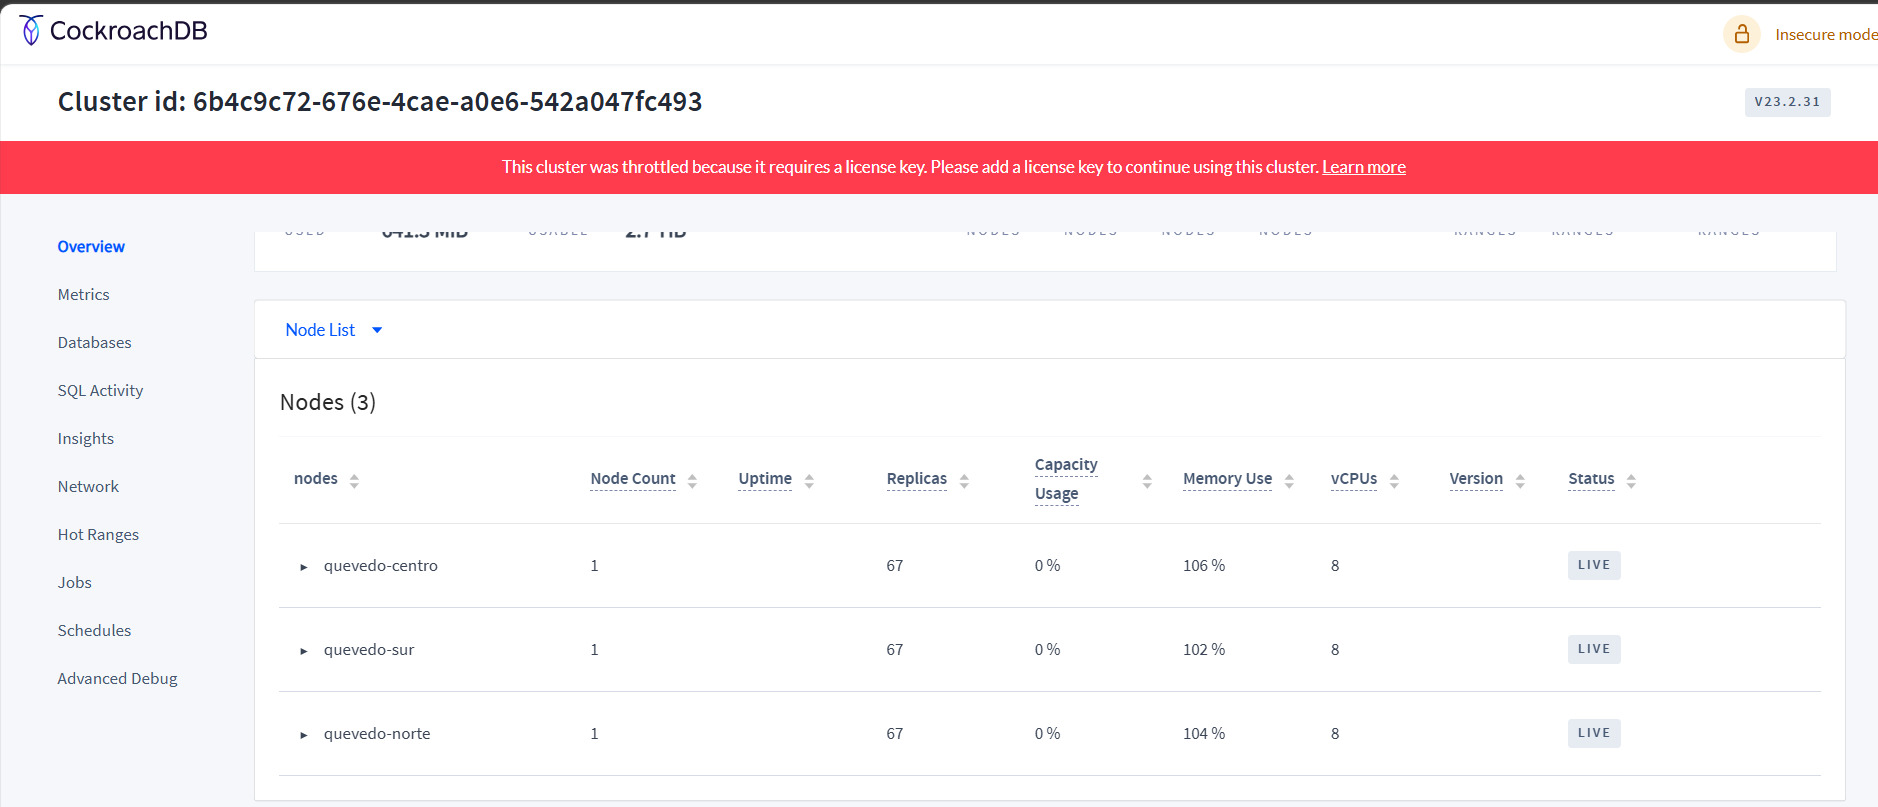
\includegraphics[width=0.85\textwidth]{dashboard.jpeg}
    \caption{Dashboard de CockroachDB mostrando los 3 nodos activos (\texttt{LIVE}), 106+ rangos replicados y 0 rangos sub-replicados.}
    \label{fig:dashboard}
\end{figure}

\subsection{Esquema del PFC y fragmentación aplicada}
\label{sec:fragmentacion-aplicada}

El esquema (Listado~\ref{lst:schema}) define \texttt{technicians} y
\texttt{tickets}, esta última con clave primaria compuesta
\texttt{(zone, id)} para que \texttt{zone} pueda usarse como clave de
partición.

\begin{lstlisting}[language=SQL,caption={Fragmento de \texttt{sql/01\_schema.sql}: tabla principal del dominio},label={lst:schema}]
CREATE TABLE tickets (
    zone            STRING NOT NULL CHECK (zone IN
        ('QUEVEDO_CENTRO','QUEVEDO_NORTE','QUEVEDO_SUR')),
    id              UUID NOT NULL DEFAULT gen_random_uuid(),
    client_id       UUID NOT NULL,
    technician_id   UUID REFERENCES technicians(id),
    category        STRING,
    priority        STRING,
    status          STRING NOT NULL DEFAULT 'NUEVO',
    created_at      TIMESTAMPTZ NOT NULL DEFAULT now(),
    sla_deadline    TIMESTAMPTZ,
    resolved_at     TIMESTAMPTZ,
    sla_breached    BOOL DEFAULT FALSE,
    PRIMARY KEY (zone, id)
);
\end{lstlisting}

La fragmentación (Listado~\ref{lst:partitions}) se aplica en un paso
independiente con \texttt{ALTER TABLE ... PARTITION BY LIST}, y cada
partición se ancla preferentemente a su nodo de localidad manteniendo
\texttt{num\_replicas=3} para no sacrificar tolerancia a fallos.

\begin{lstlisting}[language=SQL,caption={\texttt{sql/02\_partitions.sql}: fragmentación horizontal y política de zona},label={lst:partitions}]
ALTER TABLE tickets PARTITION BY LIST (zone) (
    PARTITION tickets_centro  VALUES IN ('QUEVEDO_CENTRO'),
    PARTITION tickets_norte   VALUES IN ('QUEVEDO_NORTE'),
    PARTITION tickets_sur     VALUES IN ('QUEVEDO_SUR'),
    PARTITION tickets_default VALUES IN (DEFAULT)
);

ALTER PARTITION tickets_centro OF TABLE tickets
    CONFIGURE ZONE USING num_replicas = 3,
    constraints = '{"+zone=quevedo-centro": 1}';
-- analogo para tickets_norte y tickets_sur
\end{lstlisting}

Con 20\,005 filas cargadas mediante \texttt{scripts/seed\_data.py}
(distribución objetivo 40/30/30), la distribución real observada fue:

\begin{table}[H]
\centering
\caption{Distribución real de tickets por partición tras la carga}
\label{tab:distribucion}
\begin{tabular}{@{}lrr@{}}
\toprule
Zona & Filas & \% del total \\
\midrule
QUEVEDO\_CENTRO & 8\,001 & 40.0\% \\
QUEVEDO\_NORTE  & 6\,003 & 30.0\% \\
QUEVEDO\_SUR    & 6\,001 & 30.0\% \\
\midrule
\textbf{Total} & \textbf{20\,005} & \textbf{100\%} \\
\bottomrule
\end{tabular}
\end{table}

\texttt{SHOW RANGES FROM TABLE tickets} confirmó que cada partición reside en
un rango separado, replicado en los tres nodos (\texttt{\{1,2,3\}}), lo que
verifica empíricamente las tres condiciones de corrección de la
Ecuación~\ref{eq:completitud}--\ref{eq:disjuncion}: cada fila pertenece a
exactamente una partición (disjunción), la unión de las tres particiones más
la partición \texttt{default} cubre el 100\% de las filas (completitud), y
\texttt{SELECT * FROM tickets} reconstruye la relación original sin
duplicados ni omisiones (reconstrucción).

\subsection{Prueba de tolerancia a fallos}
\label{sec:tolerancia}

Siguiendo el guion de la guía, se registró una consulta base, se detuvo
\texttt{crdb-node2}, se repitió la consulta de inmediato, se esperó 30
segundos documentando \texttt{SHOW RANGES}, y finalmente se reinició el nodo
midiendo el tiempo de reintegración. La Tabla~\ref{tab:tolerancia} resume la
evidencia recolectada (ver también el video en
\texttt{evidencia/video\_tolerancia.mp4}).

\begin{table}[H]
\centering
\caption{Cronología de la prueba de tolerancia a fallos}
\label{tab:tolerancia}
\begin{tabular}{@{}>{\raggedright\arraybackslash}p{4cm}>{\raggedright\arraybackslash}p{9cm}@{}}
\toprule
Paso & Resultado observado \\
\midrule
Consulta base (3 nodos vivos) & \texttt{COUNT(*) = 20005}, \textasciitilde{}1.5\,ms \\
\texttt{docker stop crdb-node2} & Nodo detenido \\
Consulta inmediata tras la caída & \texttt{COUNT(*) = 20005} --- responde correctamente por quórum (2 de 3 nodos) \\
\texttt{node status} con el nodo caído & \texttt{crdb-node2}: \texttt{is\_live=false}; los otros dos: \texttt{true} \\
\texttt{SHOW RANGES} tras 30\,s & Réplicas siguen listadas en \texttt{\{1,2,3\}} --- sin redistribución física; esperado, porque \texttt{server.time\_until\_store\_dead} (5\,min por defecto) aún no se cumple \\
\texttt{docker start crdb-node2} & Reinicio del nodo \\
Reintegración confirmada & \texttt{crdb-node2} vuelve a \texttt{is\_live=true} en menos de \textasciitilde{}65\,s \\
Verificación de integridad & 20\,005 filas intactas, distribución 8001/6003/6001 sin cambios \\
\bottomrule
\end{tabular}
\end{table}

La Figura~\ref{fig:raft-seq} ilustra, como diagrama de secuencia de
elaboración propia, el comportamiento interno de Raft durante este escenario:
al perderse el líder o una réplica no líder, el grupo Raft del rango afectado
sigue respondiendo mientras conserve el quórum, y solo se dispara una nueva
elección de líder si el nodo caído era efectivamente el líder de ese rango.

\begin{figure}[H]
\centering
\begin{tikzpicture}[
    thick,
    actor/.style={font=\small\bfseries},
    lifeline/.style={dashed, gray},
    msg/.style={-{Stealth}, font=\scriptsize}
]
   
    \def\cx{0}    % Cliente SQL
    \def\nix{3.5} % crdb-node1 (lider)
    \def\ntx{7.0} % crdb-node2
    \def\ntrx{10.5} % crdb-node3

    % actores
    \node[actor] (client) at (\cx,0) {Cliente SQL};
    \node[actor] (n1) at (\nix,0) {crdb-node1 (líder)};
    \node[actor] (n2) at (\ntx,0) {crdb-node2};
    \node[actor] (n3) at (\ntrx,0) {crdb-node3};

    % lineas de vida
    \draw[lifeline] (\cx,0) -- (\cx,-8);
    \draw[lifeline] (\nix,0) -- (\nix,-8);
    \draw[lifeline] (\ntrx,0) -- (\ntrx,-8);
    \draw[lifeline] (\ntx,0) -- (\ntx,-3.2);
    \draw[lifeline, red, dotted] (\ntx,-3.2) -- (\ntx,-6.0) node[midway,right,red,font=\tiny]{caído};
    \draw[lifeline] (\ntx,-6.0) -- (\ntx,-8);


    \draw[msg] (\cx,-0.8) -- node[above,font=\tiny]{\texttt{INSERT ticket}} (\nix,-0.8);
    \draw[msg] (\nix,-1.3) -- node[above,font=\tiny]{append log} (\ntx,-1.3);
    \draw[msg] (\nix,-1.7) -- node[above,font=\tiny]{append log} (\ntrx,-1.7);
    \draw[msg] (\ntx,-2.1) -- node[below,font=\tiny]{ack} (\nix,-2.1);
    \draw[msg] (\ntrx,-2.4) -- node[below,font=\tiny]{ack} (\nix,-2.4);
    \draw[msg] (\nix,-2.8) -- node[above,font=\tiny]{commit (quórum 2/3)} (\cx,-2.8);

    \node[red,font=\tiny] at (\ntx,-3.5) {docker stop crdb-node2};

   
    \draw[msg] (\cx,-4.2) -- node[above,font=\tiny]{\texttt{SELECT COUNT(*)}} (\nix,-4.2);
    \draw[msg] (\nix,-4.6) -- node[above,font=\tiny]{read (quórum 2/3, sin node2)} (\ntrx,-4.6);
    \draw[msg] (\ntrx,-5.0) -- node[below,font=\tiny]{ack} (\nix,-5.0);
    \draw[msg] (\nix,-5.4) -- node[above,font=\tiny]{resultado correcto} (\cx,-5.4);

    \node[font=\tiny] at (\ntx,-6.3) {docker start crdb-node2};
    \draw[msg, blue] (\nix,-6.8) -- node[above,font=\tiny,blue]{catch-up de log (Raft)} (\ntx,-6.8);
    \draw[msg, blue] (\ntx,-7.2) -- node[below,font=\tiny,blue]{ack, réplica al día} (\nix,-7.2);
\end{tikzpicture}
\caption{Diagrama de secuencia (elaboración propia) del comportamiento de Raft durante la caída y reintegración de \texttt{crdb-node2}: el quórum de 2/3 nodos mantiene la disponibilidad de lectura/escritura sin interrupción, y la reintegración se resuelve por \emph{catch-up} de log, no por elección de líder (porque \texttt{crdb-node2} no era el líder del rango afectado).}
\label{fig:raft-seq}
\end{figure}

\section{Resultados y análisis comparativo de rendimiento}
\label{sec:resultados}

Las cinco consultas de \texttt{sql/03\_queries.sql} se ejecutaron con
\texttt{EXPLAIN ANALYZE} cinco veces en cada entorno (clúster de 3 nodos y
nodo único), reportando la mediana para neutralizar outliers de arranque en
frío y de contención de la VM de desarrollo (metodología completa en
\texttt{evidencia/benchmark\_summary.md}).

\begin{table}[H]
\centering
\caption{Comparativa de rendimiento: clúster (3 nodos) vs. nodo único}
\label{tab:benchmark}
\begin{tabular}{@{}clrrr@{}}
\toprule
\# & Consulta & Clúster (ms) & Nodo único (ms) & Factor* \\
\midrule
Q1 & Lectura por PK & 4--5 & 2 & 0.4--0.5$\times$ \\
Q2 & Rango por zona + fecha & 7--26 & 8--11 & 0.3--1.6$\times$ \\
Q3 & Agregación cruzando zonas & 13--16 & 11--14 & 0.7--1.1$\times$ \\
Q4 & \texttt{GROUP BY} zona+categoría (SLA) & 26--29 & 34--66 & 1.3--2.3$\times$ \\
Q5 & \texttt{JOIN} tickets$\leftrightarrow$técnicos & 28--30 & 30--61 & 1.1--2.0$\times$ \\
\bottomrule
\end{tabular}

\vspace{0.2cm}
\footnotesize *factor = tiempo\_nodo\_único / tiempo\_clúster (>1 significa que el clúster fue más rápido). Rangos observados entre dos corridas independientes de 5 mediciones cada una; ver \texttt{evidencia/resultados.csv} para los datos crudos.
\end{table}

\textbf{Interpretación.} El patrón es consistente con la teoría del
Capítulo~\ref{sec:teoria}: en Q1 (lectura puntual por clave primaria), el
nodo único gana porque no hay trabajo que paralelizar --- el único costo es
la coordinación del quórum Raft, que el nodo único no paga. En Q4 y Q5, las
consultas con más trabajo de cómputo (agregación sobre 20\,000 filas y
\emph{join}), el plan distribuido del clúster (\texttt{nodes: n1, n2} en el
\texttt{EXPLAIN ANALYZE}) sí aporta paralelismo real y el clúster gana con
margen consistente. Q2 y Q3 quedan en un punto intermedio donde el resultado
depende de si la consulta toca una sola partición (Q2, favorece al clúster
por localidad de partición) o cruza las tres (Q3, cercano al empate). Esto
confirma que, a este volumen de datos (20\,000 filas), la ventaja de la
distribución no es universal sino que depende del tipo de consulta ---
observación que sería clave para dimensionar cuándo migrar a un clúster de
más de un nodo en un escenario de producción real del PFC ACC.
\section{Preguntas de análisis obligatorias}
\label{sec:analisis}

\subsection*{1. ¿Cómo garantiza CockroachDB consistencia ante la caída de un nodo?}

CockroachDB divide el espacio de claves en rangos (\emph{ranges}) y replica
cada uno en un grupo Raft independiente, típicamente de tres réplicas
\cite{taft2020}. Dentro de cada grupo, Raft elige un líder por mayoría;
solo el líder acepta escrituras nuevas, las anexa a su log replicado y las
propaga a los seguidores \cite{ongaro2014}. Una escritura se confirma
únicamente cuando la mayoría de las réplicas del rango ha persistido esa
entrada del log (en un grupo de tres, dos de tres), lo que impide que
dos líderes comprometan simultáneamente entradas conflictivas para la misma
posición del log \cite{ongaro2014}. En la prueba de la
Sección~\ref{sec:procedimiento}, al detener \texttt{crdb-node2}, cada rango
en el que este participaba perdió una réplica, pero mientras el nodo caído
no fuera el líder de un rango dado, ese rango siguió respondiendo gracias al
quórum de 2/3 restante. Si hubiera sido líder, los seguidores habrían
detectado la ausencia de \emph{heartbeats} y disparado una nueva elección en
cuestión de segundos. Ningún dato se pierde porque toda escritura confirmada
ya estaba persistida en al menos dos réplicas antes de reportarse exitosa al
cliente; al reintegrarse el nodo (\textasciitilde{}65\,s en la prueba),
simplemente recibe del líder las entradas de log que le faltan, sin
intervención manual \cite{taft2020,ongaro2014}.

\subsection*{2. CockroachDB (serializable) vs. Cassandra (consistencia eventual): ¿cuál para el PFC ACC?}

Para el dominio de ACC, la elección correcta es CockroachDB, y el modelo
PACELC de Abadi explica por qué \cite{abadi2012}. Cassandra prioriza
disponibilidad y baja latencia incluso a costa de consistencia, con un
modelo eventual ajustable por nivel de quórum de lectura y escritura
\cite{lakshman2010}, adecuado para casos donde una lectura ligeramente
obsoleta es tolerable, como un contador de \emph{likes}. Pero en ACC la
operación crítica es la asignación de un ticket a un técnico: bajo
consistencia eventual, dos técnicos podrían leer simultáneamente el mismo
ticket como disponible y ambos intentar tomarlo, generando doble trabajo o
dejando sin asignar un ticket con SLA crítico. CockroachDB evita esto por
diseño, al implementar aislamiento serializable estricto, apoyado en
\emph{timestamps} de reloj híbrido y en el orden total que impone Raft
dentro de cada rango \cite{taft2020}. En términos de PACELC, esto significa
que incluso sin partición de red (rama \emph{Else}), CockroachDB elige
sistemáticamente consistencia sobre latencia: acepta una escritura algo más
lenta(el costo del \emph{round-trip} del consenso Raft) a cambio de
que \texttt{ticket-service} nunca necesite lógica de resolución de
conflictos en el cliente, algo que sí sería obligatorio con Cassandra. Dado
que el volumen de escrituras de un ISP regional es modesto frente a la
escala geo-distribuida para la que Cassandra fue pensada, ese costo de
latencia adicional es aceptable y la ganancia en simplicidad y corrección lo
justifica ampliamente \cite{viotti2016}.

\subsection*{3. Diseño de la fragmentación horizontal explícita para \texttt{tickets}}

La estrategia implementada usa \texttt{PARTITION BY LIST} sobre la columna
\texttt{zone}, con las particiones \texttt{tickets\_centro},
\texttt{tickets\_norte}, \texttt{tickets\_sur} y una partición
\texttt{DEFAULT} de resguardo para valores no anticipados. Se eligió
\texttt{LIST} y no \texttt{RANGE} porque \texttt{zone} es un conjunto
pequeño, fijo y discreto de tres categorías sin relación de orden entre
ellas; \texttt{RANGE} tiene sentido para claves continuas y ordenables, por
ejemplo particionar por la fecha de creación para descartar datos antiguos,
pero forzar un orden artificial sobre zonas geográficas no relacionadas
habría sido semánticamente incorrecto \cite{ge2024,mehta2022}. La columna
\texttt{zone} se incluyó además en la clave primaria compuesta junto al
identificador, un requisito técnico de CockroachDB para que cada fila
pertenezca inequívocamente a una sola partición sin tener que reevaluar el
predicado en cada operación. La justificación de negocio es que el patrón
de acceso dominante de \texttt{ticket-service} (un técnico consultando
los tickets de su propia zona) alinea el filtro más común con la clave de
partición, lo que, como se observó en la consulta Q2 de la
Sección~\ref{sec:resultados}, permite resolver la consulta tocando un solo
rango en vez de dispersar la lectura entre las tres particiones. Cada
partición además se ancla mediante \texttt{CONFIGURE ZONE} con una
restricción de localidad hacia el nodo de su misma zona, acercando el
cómputo a donde probablemente se originan las lecturas más frecuentes, sin
renunciar a las tres réplicas completas que exige la tolerancia a fallos del
clúster \cite{taft2020}.

\subsection*{4. Atomicidad de transacciones multi-tabla en distintos nodos}

Cuando una transacción de ACC modifica átomicamente filas en rangos
distintos (por ejemplo, el estado de un ticket y un contador de carga de
un técnico) CockroachDB no depende de un protocolo de \emph{commit} en
dos fases clásico entre nodos independientes, sino que compone la
atomicidad a partir de Raft y de un protocolo transaccional propio
\cite{taft2020}. Uno de los rangos involucrados se designa como registro
transaccional, donde se anota el estado de la transacción como pendiente,
confirmada o abortada. Cada escritura individual se propone primero como un
valor provisional o \emph{intent}, replicado con las garantías normales de
Raft dentro del grupo de su propio rango, de forma independiente y en
paralelo con los demás rangos afectados \cite{taft2020,ongaro2014}. Solo
cuando todos los \emph{intents} han sido comprometidos por el quórum Raft de
su rango correspondiente, el coordinador marca el registro transaccional
como confirmado; los \emph{intents} se resuelven después de forma
asíncrona, y cualquier lector que los encuentre antes puede consultar ese
registro para saber si debe considerarlos válidos. Si el coordinador falla a
mitad de camino, cualquier otro nodo que lea un \emph{intent} puede, tras un
tiempo de espera, resolver la transacción consultando el registro, evitando
el bloqueo indefinido característico del \emph{commit} en dos fases clásico
\cite{skeen1981}. En suma, la atomicidad multi-tabla se logra componiendo
varias instancias de consenso Raft bajo un único registro transaccional como
fuente de verdad, no mediante un coordinador central que deba permanecer
vivo \cite{taft2020}.

\section{Análisis crítico}
\label{sec:analisis-critico}
La verificación experimental confirmó lo que predice la teoría de la
Sección~\ref{sec:teoria}: el clúster resistió la caída de un nodo sin dejar
de funcionar y sin perder información, tal como se espera del algoritmo
Raft cuando se mantiene la mayoría de los nodos activos, es decir, un
quórum de 2 de 3 \cite{ongaro2014}. Sin embargo, al medir el rendimiento
apareció un matiz que la teoría por sí sola no deja ver con claridad: con
20\,000 filas, el clúster distribuido no siempre fue más rápido que una
sola instancia de base de datos, sino que esto dependió del tipo de
consulta que se ejecutara. Esto coincide con lo que plantea Abadi sobre
que todo sistema distribuido paga un costo de tiempo por mantener la
información consistente entre nodos, incluso cuando no hay ningún
problema de red de por medio \cite{abadi2012}: ese costo, que implica que
los nodos se pongan de acuerdo entre sí antes de confirmar cada
operación, se nota más en consultas simples (como buscar un ticket
por su identificador) y se compensa solo cuando la consulta requiere
suficiente trabajo como para que repartirlo entre varios nodos realmente
ayude. Una limitación real de esta práctica es que se realizó en un
entorno de desarrollo local (contenedores Docker en una sola máquina),
donde los tres nodos comparten el mismo procesador, disco y red que el
propio cliente que hace las consultas; en un despliegue real con los
nodos ubicados en distintas regiones (el escenario para el que
CockroachDB fue pensado) es de esperar que la ventaja de distribuir
los datos sea mayor en consultas que aprovechan la localidad de la
partición (Q2), y que el costo de mantener consistencia se sienta más en
el tiempo que toma la comunicación entre regiones que en el procesamiento
local. Para el PFC ACC, la recomendación práctica que se desprende de
este análisis es priorizar el diseño de índices y particiones alineados
con los patrones de consulta reales del sistema (como ya se hizo con
\texttt{zone}), en lugar de asumir que "más nodos" es automáticamente
"más rápido" para cualquier tipo de consulta.

\section{Conclusiones}
\label{sec:conclusiones}

Se implementó y verificó experimentalmente un clúster CockroachDB de tres
nodos aplicado al esquema del PFC ACC, demostrando fragmentación horizontal
por zona con las tres condiciones de corrección satisfechas, tolerancia a
fallos por quórum Raft sin pérdida de datos ante la caída de un nodo, y una
ganancia de rendimiento distribuido que es real pero dependiente del tipo de
consulta, no universal. El ejercicio confirma que la teoría de bases de
datos distribuidas (fragmentación, replicación, consenso y los
trade-offs de PACELC) no es solo material de examen, sino que se puede
observar directamente en el comportamiento medible de un sistema real.

\subsection*{Conclusiones individuales}

\paragraph{Jhinson Stalyn Aucatoma Celorio:} En esta práctica se pudo comprobar que la fragmentación de datos, un concepto que en el fundamento teórico se presenta como un objetivo de diseño, realmente funciona en un sistema como CockroachDB sin complicar el uso de la base de datos. Al dividir la tabla de tickets por zona (centro, norte y sur de Quevedo), se pudo verificar que cada partición se guardaba correctamente en el clúster y que las consultas seguían funcionando igual que si la información estuviera en un solo lugar. Este proceso confirma que la teoría sobre fragmentación tiene una aplicación concreta y medible. Además, se pudo evidenciar que no fue necesario crear una base de datos nueva para el PFC ACC, sino que se reutilizó el esquema ya existente del sistema de tickets, adaptándolo al entorno distribuido. Esto demuestra que estos conceptos pueden aplicarse de forma progresiva sobre un sistema ya construido, sin tener que rediseñarlo por completo.

\paragraph{Jeremy Alexis Alvarez Parraga:} Con la prueba de tolerancia a fallos llevada a cabo de manera práctica pudo mostrar algo que antes solo se veía de forma teórica: cuando uno de los tres nodos del clúster se detiene, el sistema sigue funcionando siempre que los otros dos continúen de acuerdo entre sí, es decir, mientras se mantenga la mayoría o "quórum". Al detener el nodo crdb-node2, las consultas siguieron respondiendo correctamente y no se perdió información, lo cual respalda directamente lo estudiado sobre el algoritmo Raft. También se observó que, después de 30 segundos con el nodo caído, el sistema no reorganizó de inmediato la información entre los nodos restantes, y esto tiene una explicación sencilla: el clúster espera varios minutos antes de asumir que un nodo está definitivamente fuera de servicio, para no reaccionar de más ante fallas breves o temporales. Cuando el nodo se reinició, se puso al día con la información faltante en menos de un minuto, sin necesidad de elegir un nuevo líder. Todo esto demuestra que un sistema como el de ACC podría mantenerse disponible incluso ante fallas de hardware o de red.

\paragraph{Carlos Jose Carpio Mendoza:} Al comparar el rendimiento del clúster distribuido frente a una sola instancia de base de datos, se pudo descubrir que tener más nodos no siempre significa mayor velocidad. En la consulta más simple, buscar un ticket por su identificador, la base de datos de un solo nodo fue más rápida, porque no hay ninguna tarea que se pueda repartir entre varios nodos y, en cambio, el clúster sí debe invertir tiempo en que los nodos se pongan de acuerdo entre sí. En cambio, en consultas más exigentes, como calcular estadísticas por zona y categoría, o relacionar tickets con técnicos, el clúster resultó ser claramente más rápido, porque ahí sí puede repartir el trabajo entre varios nodos al mismo tiempo. Esto confirma la idea de que mantener la información siempre consistente entre nodos tiene un costo, y que ese costo solo vale la pena cuando la consulta implica suficiente trabajo como para aprovechar la distribución. Para el PFC ACC, esto sugiere que antes de adoptar un clúster distribuido conviene analizar bien qué tipo de consultas se van a ejecutar con más frecuencia.

\section*{Declaración de uso de inteligencia artificial generativa}
\label{sec:declaracion-ia}

En la elaboración de este informe se utilizó un asistente de inteligencia
artificial generativa (Claude, de Anthropic) como herramienta de apoyo, no
como autor del contenido técnico. Su uso se limitó a tres propósitos
concretos. Primero, la verificación de las referencias bibliográficas
citadas en el fundamento teórico, confirmando que los DOI e ISBN
correspondieran efectivamente a la fuente citada y que las editoriales
fueran de origen académico reconocido, descartando fuentes depredadoras o no
arbitradas. Segundo, el apoyo en la redacción del Análisis crítico
(Sección~\ref{sec:analisis-critico}), las Preguntas de análisis obligatorias
(Sección~\ref{sec:analisis}) y las conclusiones individuales
(Sección~\ref{sec:conclusiones}): en los tres casos, las ideas, los
hallazgos y las conclusiones fueron redactados originalmente por los
integrantes del equipo a partir de su propia experiencia con el desarrollo
de la práctica y de la evidencia experimental obtenida; la herramienta se
empleó únicamente para mejorar la coherencia, la fluidez y la conexión entre
oraciones del texto ya elaborado por los integrantes, sin introducir
afirmaciones, datos o interpretaciones nuevas. Tercero, se usó de forma
puntual para revisar la consistencia gramatical general del documento. En
ningún momento la IA generó por sí sola resultados experimentales, código de
implementación ni las cifras del análisis comparativo de rendimiento.

\clearpage
\printbibliography

\end{document}
